
Simultaneous Multi-Threading reprezinta cea mai avansata forma de arhitectura superscalara. Pentru
a verifica avantajale ei, am inclus un benchmark din articolul \cite{tuck2003initial}.

In acel test, se verifica cat de mult poate mari viteza de executie folosind SMT. Dupa cum se
observa pe rezultate, speedup-ul mediu este de aproximativ 1.2. Exista cazuri in care speedup-ul
este sub 1, dar sunt rare. Acest test arata ca prin dublarea registriilor si folosirea arhitecturii
superscalare deja existentente, o marirea de aproximativ 5\% a unui nucleu rezulta intr-o crestere
a performantei de pana la 40\%.

\begin{figure*}[ht] \centering
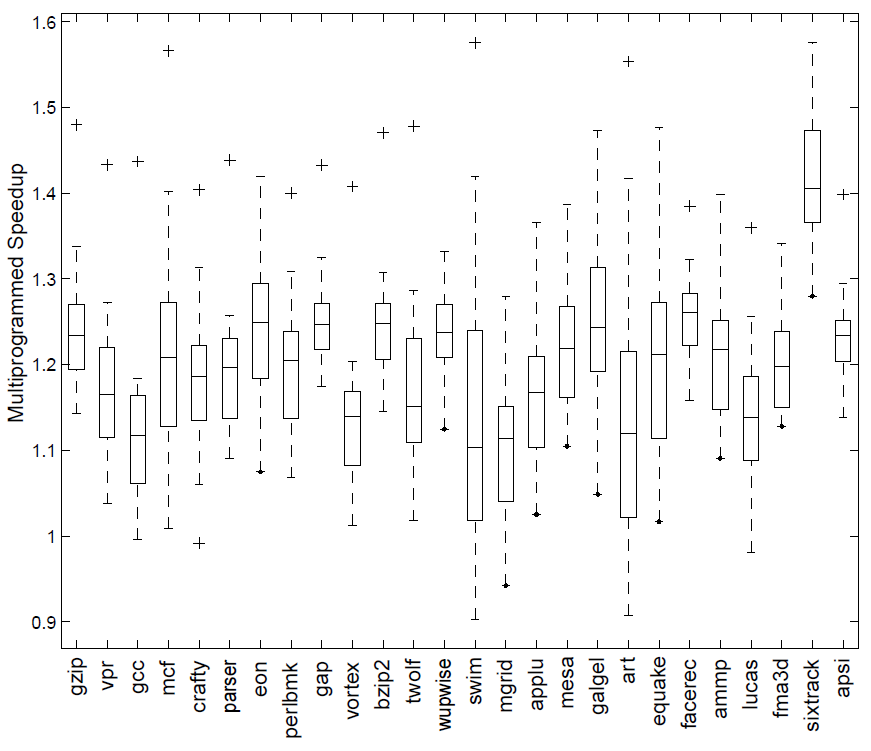
\includegraphics[width=0.9\textwidth]{img/smt.png}
\caption{Speed-up obtinut folosit SMT} \end{figure*}

